\chapter{The decisions that mattered}

\section{Reconstructing both visits together}

Covered in Section~4.2. The single most important choice in the project, and the one worth being
able to defend in detail.

\section{Tracking empty space, not just full space}

The thing that stops occlusion being reported as change. Without it the system would be a
difference detector rather than a change detector, and on real footage the difference between
those two is most of the room.

\section{Refusing to answer when the evidence is missing}

The system will miss real changes in parts of the room that only one visit covered. That is
intended, not an oversight.

For a robot, a missed change is a wasted detour. A hallucinated clear path is a collision. Given a
choice between the two failure modes, this one is correct.

\section{Refusing to name things it cannot see properly}

An early version of the report confidently announced that a television had moved. It had not.
There was no television. CLIP was guessing, at a confidence barely distinguishable from random
chance, and the program was printing those guesses as fact.

\begin{plainbox}
With twenty nine candidate labels, a model with no idea scores about $1/29 = 0.034$ for its best
guess. The actual scores coming back were $0.035$. The model was not choosing, it was shrugging.
\end{plainbox}

There is now a floor. Anything scoring near chance is reported as ``unidentified object'', and
moves are not paired on a name nobody believes. The output went from six invented findings to ten
honest ones.

\begin{watch}
This is worth noticing as a general lesson. The system was not broken. It was producing output
that looked exactly like a working system, and only checking the confidence numbers revealed that
the labels were noise.
\end{watch}

\section{Testing against a known answer}

Rather than filming a room and eyeballing the output, the project includes a program that draws a
fake room where the changes are scripted in advance. That makes the results checkable rather than
merely plausible.

\begin{figure}[h]
\centering
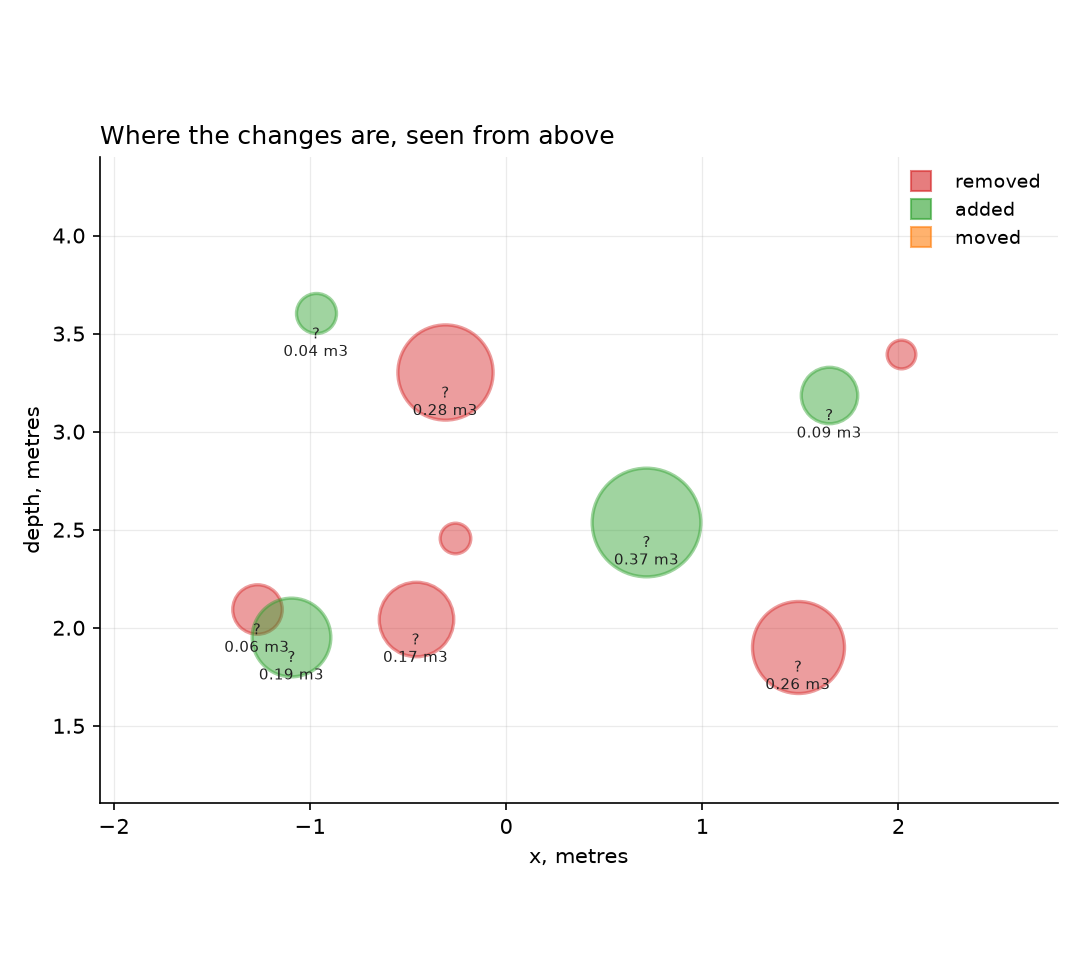
\includegraphics[width=0.92\textwidth]{topdown.png}
\caption{The detected changes seen from above, circle size proportional to volume. The four real
changes land in four different parts of the room, which is what a result tracking real geometry
looks like. A result driven by camera motion would pile up in one corner.}
\end{figure}

\begin{figure}[h]
\centering
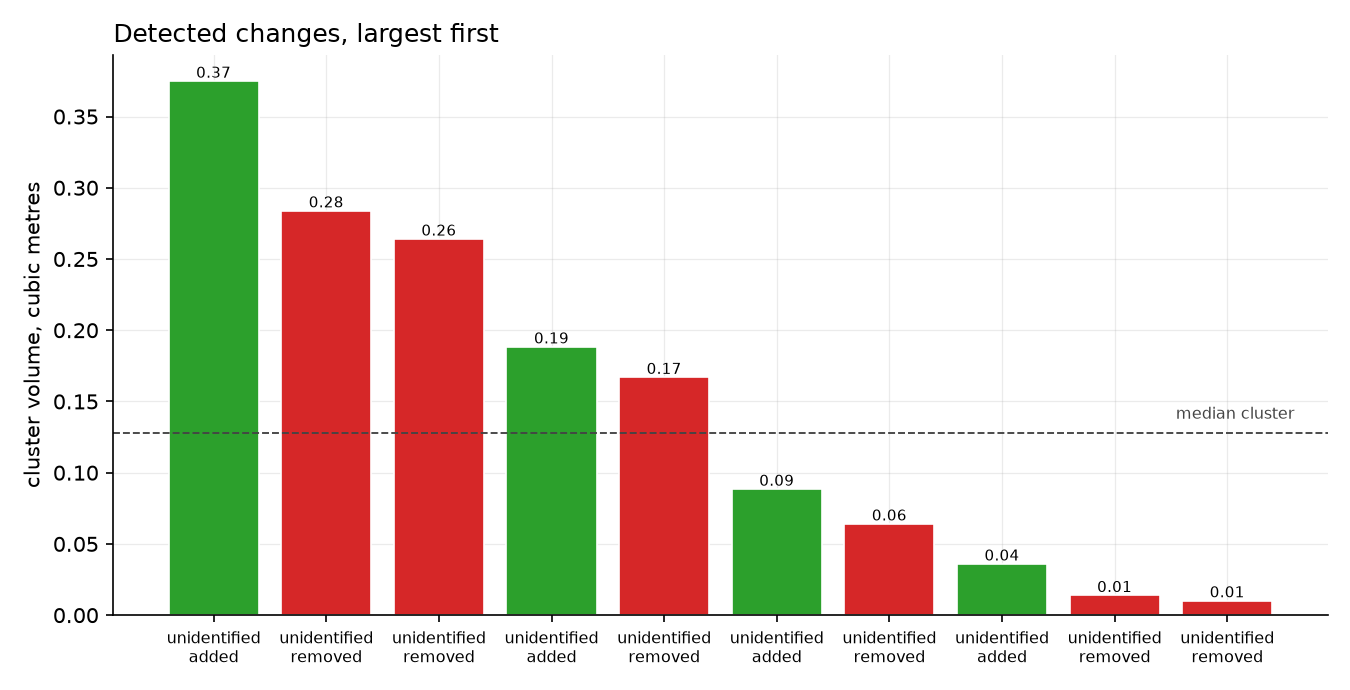
\includegraphics[width=\textwidth]{change_summary.png}
\caption{Every detected cluster by volume. The four real changes are the four largest. Everything
below the median line is depth error on flat walls rather than an object, and it is why a minimum
cluster size exists in the configuration.}
\end{figure}
